
\normalfont\normalsize
\chapter{Sparrow R}

Most of the nodes are build using the AVR processor
\cite{currentnodes}\cite{voinescu2013lightweight}, an 8-bit architecture. Few attempts have been made
using the newer ARM Cortex-M3 32-bit architecture. The benefits of higher computing power are presented here
\cite{jurdak2011opal}, where a 4.6 throughput can be obtained compared to an 8-bit CPU over the
same wireless network. Unfortunately, the downside is higher power consumption that can create
difficulties for certain power supplies. Even though the same average power consumption can be obtained, due
to higher power peaks, the voltage of the power supply can drop to a lower level than the minimum
required voltage of the node.

The current nodes, Sparrow V3.2 and SparrowV4, use an AVR 8-bit architecture and run at a speed of
16MHz. For our solar powered node, we wanted to use a newer, more powerful and lower power
microcontroller. Based on the previous requirements, we have chosen an ARM Cortex-M0+ 32-bit Atmel SamR21.


\section{\textit{Performance}}

We present bellow the main differences between the two MCUs, SamR21 and ATmega128RFA1\cite{atmegafa}.

\begin{table} \centering
\begin{tabular}{llr}
\hline
Criteria    & Atmega128RFA1 & SamR21 \\
\hline
CPU Speed      & 16 MHz    & 48 MHz      \\
CPU architecture      & AVR 8bit    & Cortex M0+ 32bit      \\
CPU Power          & 4.1 mA       & 6.5 mA       \\
Flash           & 128 kB        & 256 kB        \\
RAM                 & 16 kB     & 32 kB         \\
Flash Endurance     &  50000    & 150000        \\
Rx Consumption       & 12.5 mA     & 11.8 mA     \\
Tx Consumption       & 14.5 mA @ 3.5mA     & 13.8 mA @ 4 dBm      \\
Receiver sensitivity & -100 dBm      & -101 dBm       \\
Tx Max Power & 3.5 dBm      & 4 dBm       \\
Package & QFN64      & QFN48 or QFN32      \\
\hline
\end{tabular}
\caption{Comparison between Atmega128RFA1 and SamR21}
\end{table}

\begin{table} \centering
\begin{tabular}{llllr}
\hline
Criteria    & Atmega128RFA1 & SamR21 & Total Advantage & Advantage per MHz \\
\hline
Integer Iterations      & 44890    & 403950   & 8.99 &  2.99 \\
Branch Iterations      & 27782    & 93552  &  3.36 &  1.12  \\
While(1) Iterations          & 191536     & 6693086    & 34.94  & 11.64  \\
\hline
\hline
\end{tabular}
\caption{Speed comparison}
\end{table}

\begin{table} \centering
\begin{tabular}{llr}
\hline
Criteria    & Atmega128RFA1 & SamR21 \\
\hline
Integer Iteration    &  274 nJ & 49 nJ \\
Branch Iteration      & 442 nJ & 208 nJ  \\
While(1) Iteration          & 64 nJ & 2.9 nJ \\
\hline
\hline
\end{tabular}
\caption{Energy efficiency comparison}
\end{table}

Being a 32-bit architecture, even though SamR21 consumes 5.5mA
compared to 4.1mA of the Atmega128RFA1, for simple 32-bit integer addition, the SamR21 consumes only 49nJ
per iteration while the 8-bit microcontroller consumes 274nJ (almost 5 times more). Considering
performance figures, the SamR21 was 9 times faster with 403950 iterations per second while
Atmega128RFA1 managed only 44890 iterations.

Testing the performance of the branch predictor, revealed that the M0+ is only 12\% better than
the older 8-bit counterpart when running at the same speed, but thanks to the frequency difference,
it ends up being 3.36 times faster.


\begin{figure}[ht] \centering
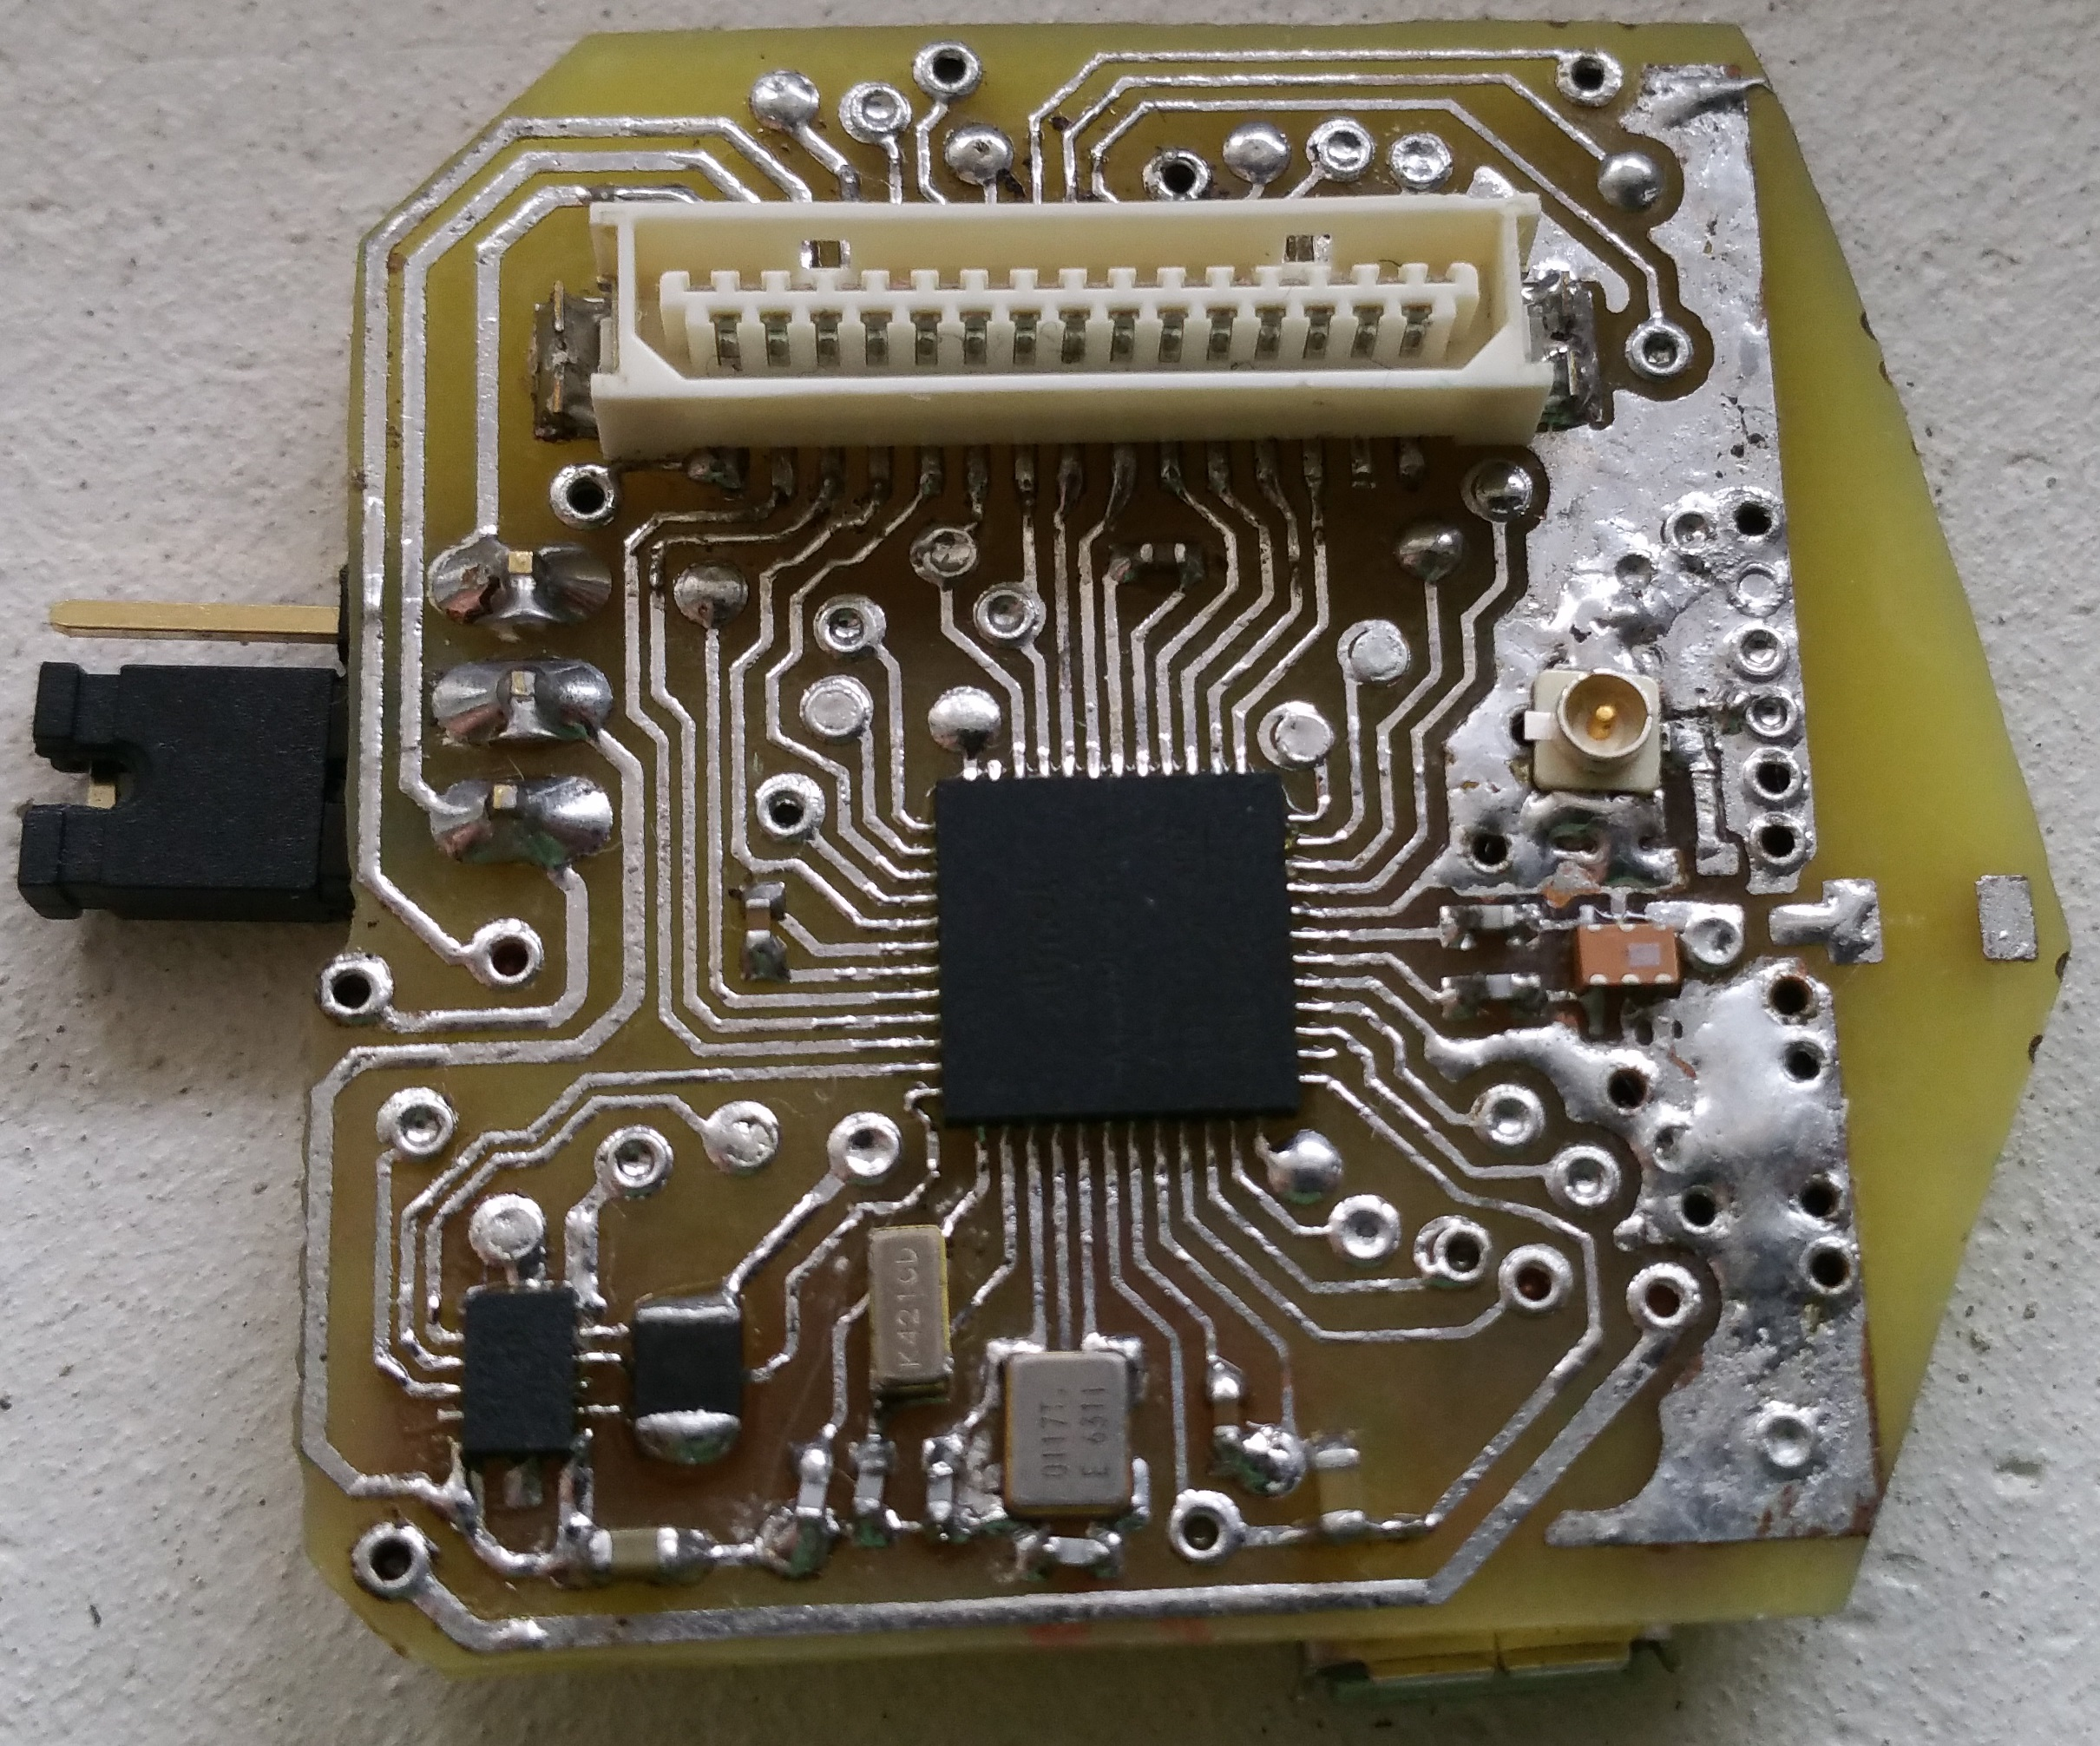
\includegraphics[width=0.85\textwidth]{img/sparrowrf.jpg}
\caption{Sparrow R node}
\end{figure}

The SamR21 microcontroller is almost the same as SamD21 \cite{samd21}, which is used in the Arduino
Zero boards. This allowed us to use exiting code, but unfortunately a not well
written one.

Even thought the Arduino software is well designed, it was not designed with low power consumption
in mind. We will describe some of the problems encountered in the current software stack.

The first problem we noticed was that the Arduino Zero board had no sleep functionality implemented.
The ideal idle current consumption should have been less than 5$\mu$A, tested and measured using a
project created in Atmel Studio 7.0. The current consumption of the board was around 350${\mu}$A. Further
tests revealed that the USB device was always initialized, which accounted for the extra
200${\mu}$A.
The remaining of 150${\mu}$A came from a default initializations of the pins as input pins, but this only
lowered the current consumption to about 60${\mu}$A. We kept searching for a cause, and discovered that
the clock generators are never disabled at start-up, which accounted for about 30${\mu}$A.

So far we managed to a decrease the idle current consumption for the platform from 350${\mu}$A to about
30${\mu}$A @ 3.2V, but it is still far from ideal. Surprisingly, lowering the voltage from 3.2V to 1.8V lead
to  decrease in sleep current consumption down to 3.3${\mu}$A. When examining the power trace using a digital oscilloscope, we found
that a very low frequency clock remains active, which at 3.2V has high spikes in power consumption.

Though we did not reach the goal of 5${\mu}$A, we still managed a respectable 30${\mu}$A @ 3.2V and
less than 4${\mu}$A @1.8V.
Due to time constrains and the need to use the nodes in order to implement and test new
features, we decided that for now this is acceptable, and for future revisions, we will come back
and find the extra clock source.

Even the run current consumption was not ideal, instead of achieving the promised 70${\mu}$A/MHz @ 3.2V,
or around 3.5mA @ 48MHz, the microcontroller consumed 8mA @ 48MHz. We managed to reduce the current consumption to 5.5mA @ 48MHz, due to
clock optimizations presented bellow.

The first modification was to change the clock of the peripheral interfaces, instead of 48 MHz, we run them at 12 MHz.
Also if peripherals are not used, we completely disable them. Due to this, we ran into problems
related to SERCOM implementation, a generic module that handles USART, SPI and I2C. It was working
on Arduino Zero, because the CPU and the BUS were configured to run at the same speed, but because of
previous clock source modifications, the SERCOM did not set the correct speed. Also, there are 6
SERCOMs, and instead of enabling the clock for each one only when it is used, all of them were
enabled, which lead to extra power consumption during run time.

\begin{figure}[ht] \centering
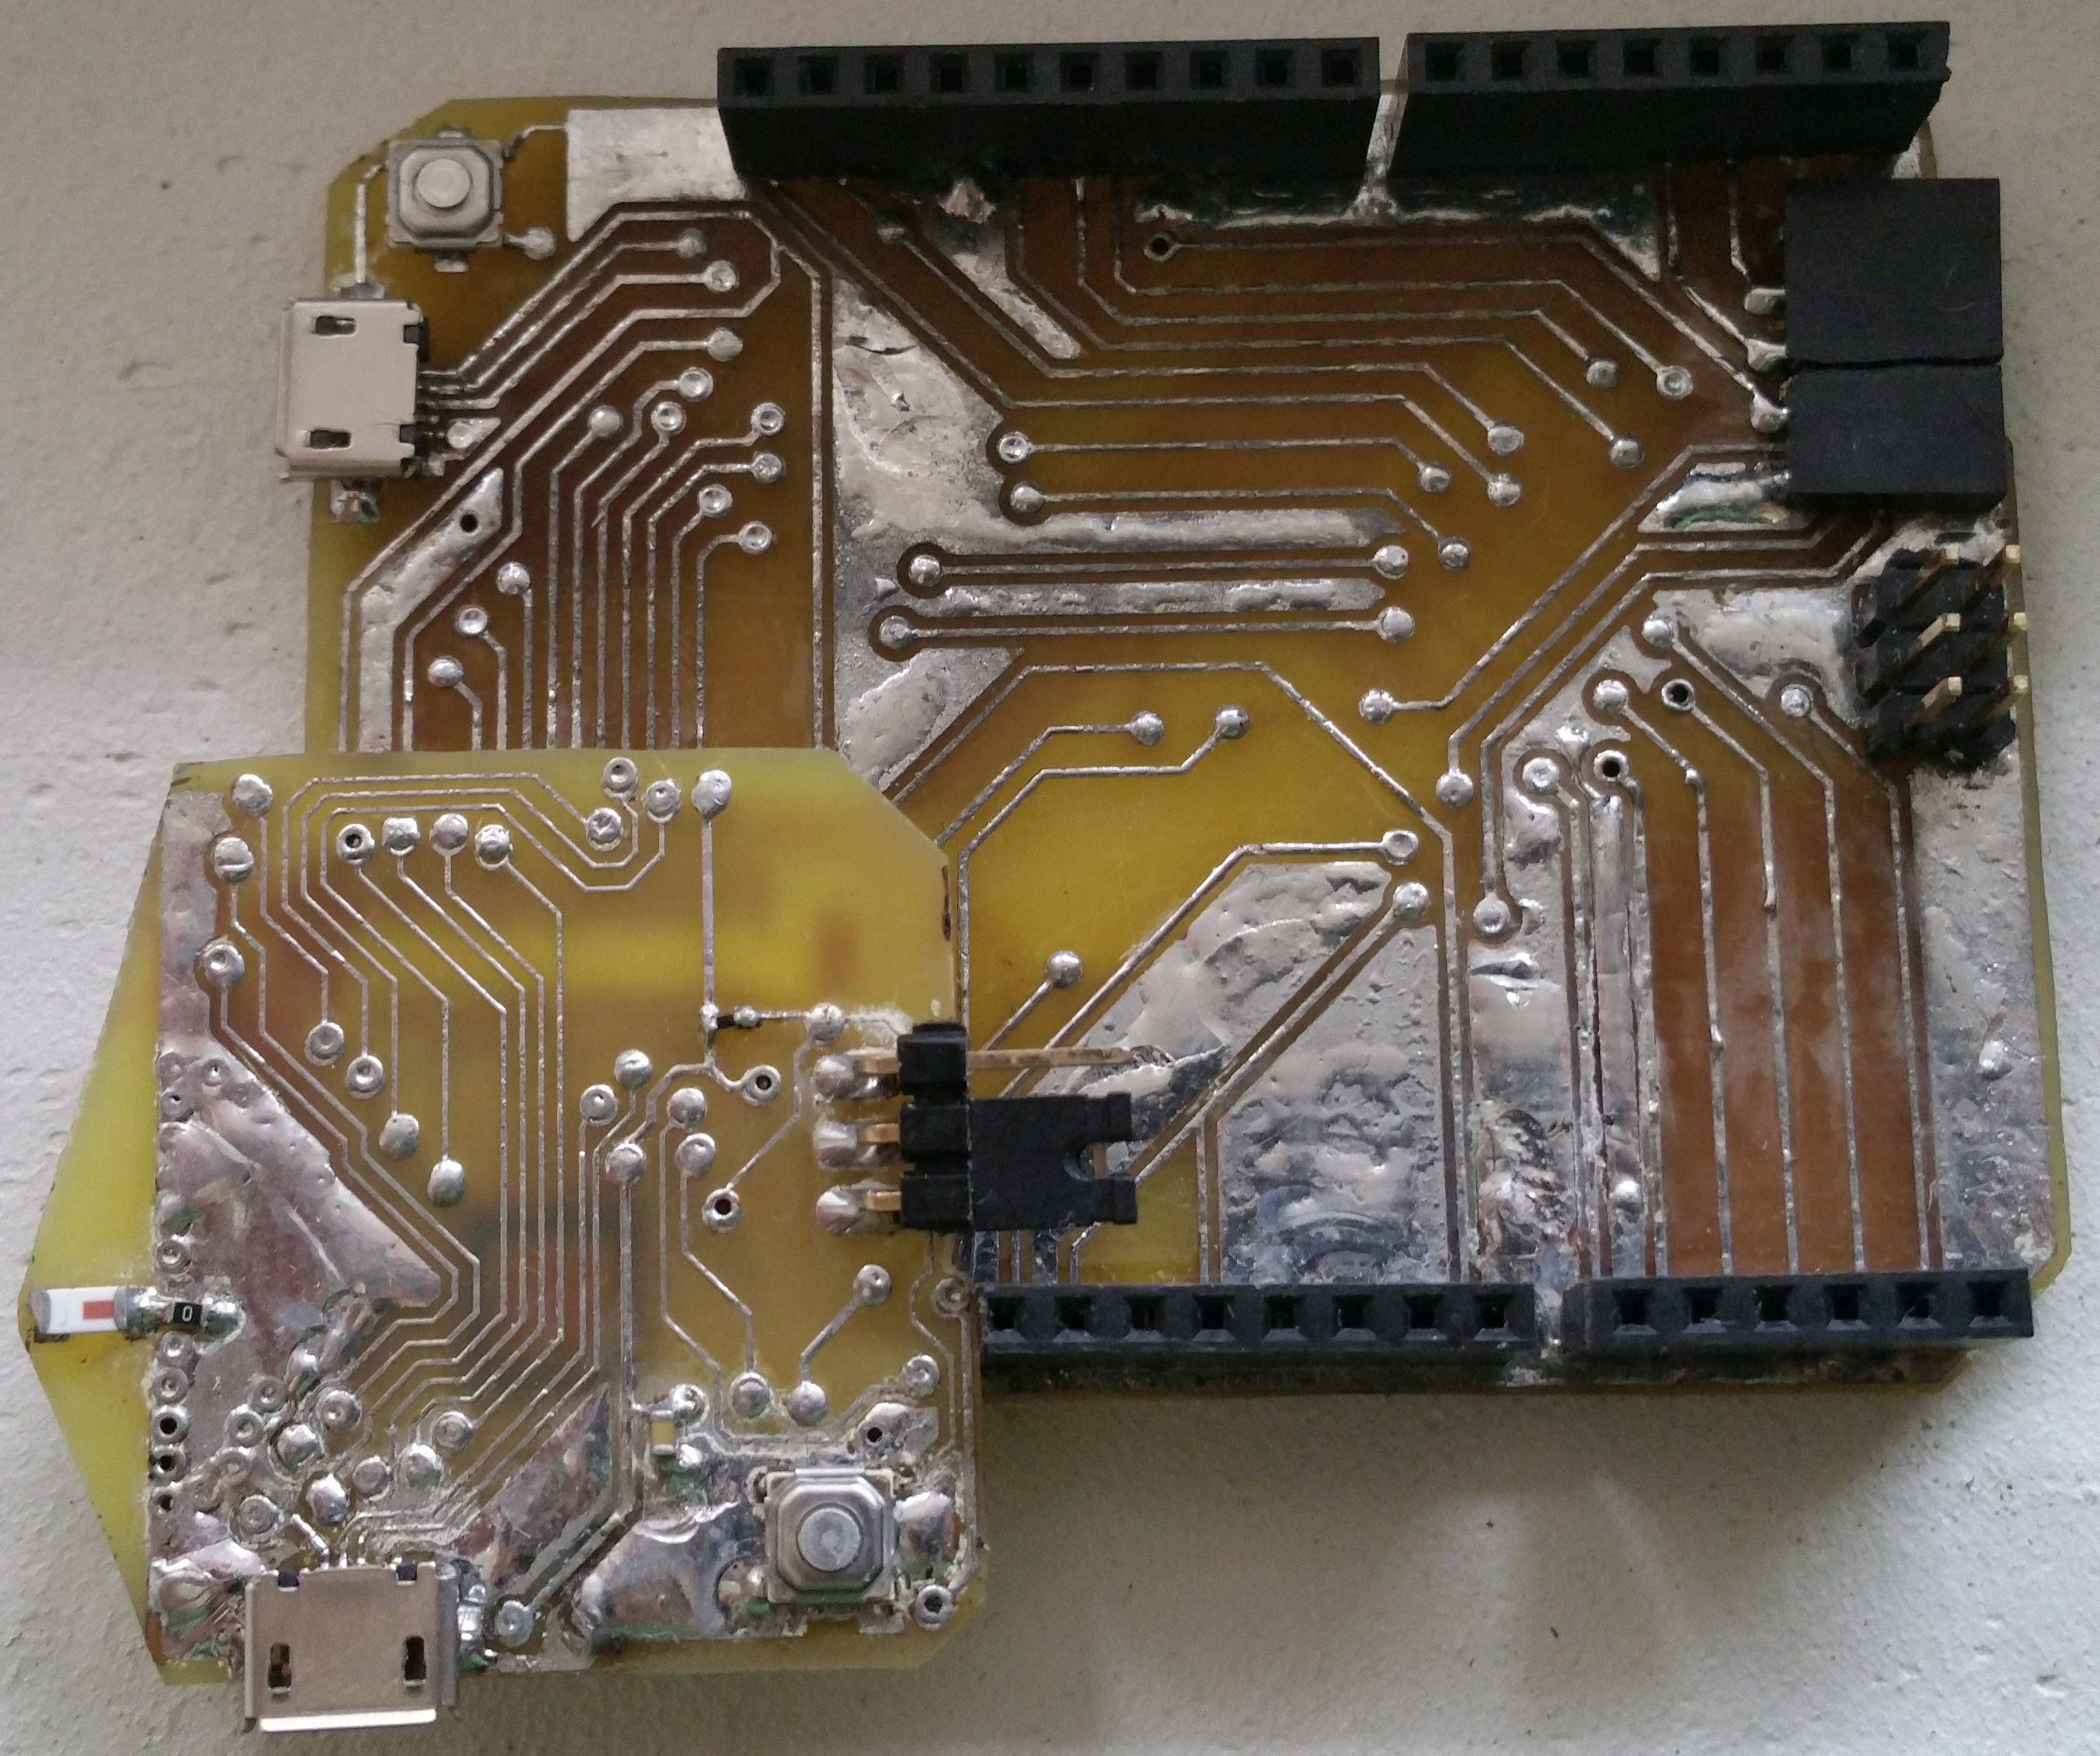
\includegraphics[width=0.85\textwidth]{img/base-with-sensor.jpg}
\caption{Sparrow R node mounted on Aduino compatible base}
\end{figure}

\section{\textit{Hardware}}
Because not all sensors are designed to run at 1.8V up to 3.2V, we need to be able to dynamically
change the operating voltage of the node. We used the TPS62742, a step-down switching DC/DC converter
with up to 90\% efficiency, voltage selectable output from 1.8V to 3.2V in 200mV steps, 360nA
quiescent current and a special MCU controllable load output, with push-pull transistors. In
inactive state the load line is pulled to GND and when active is pulled to VCC. When active it
consumes 12${\mu}$A, but compared to the controlled sensors, this should not be noticeable. Because this
allows to completely power down the sensors, the "stand-by" current consumption is 0${\mu}$A and it also
eliminates the previous design problem of floating GND which allowed the sensors to "steal" power
from other pins and not be properly disabled.

The node can be connected to an extension daughter board which fully respects the Arduino pinout.
The advantage of this approach is that it allows to easily test and prototype new configurations in
order to prepare the project in the shortest time possible. Also existing hardware designed for Arduino can work with this board,
which increases the number of compatible hardware. In total, 20 I/O pins are available, pins that
can be used for connecting sensors, either on the daughter board, or directly on a specially
designed board.

A jumper can select whether the Node is powered from USB or from other 2.1V+ voltage supplies. Through
the same jumper a power measuring device can be used to monitor the total power consumption. In case the DC/DC converter is not
needed the node can use other power sources.

\section{\textit{Software}}

We implemented new modules designed for low power like sleep and power management, which can dynamical
change the running voltage between 1.8V to 3.2V when requested, enable or disable the LOAD power
line. This allows the user to select which voltage is better required for applications. For example,
some sensors must be powered at exactly 2.8V while others at 2.5V or lower. Using this module, the
user can select the desired voltage, use the sensors and then switch to the lowest
voltage in order to obtain the best power consumption possible.

The RF module is an AT86RF233, integrated into the microcontroller. We desired to create an easy to
use software stack, that will let the user focus on what to do with the platform and not how to do
it. We integrated the module for the RF in the core of the platform, module based on this Arduino
library \cite{rf233}. Furthermore, we added extra features and fixed the existing bugs of the
library. For example, in case the RF is constantly running in receive mode for
more than 5 minutes, it is recommended to do Fine Tuning of the PLL clock in order to eliminate
possible clock skews. Feature wise, when the module automatically receives a packet, it saves it
locally together with the RSSI and LQI, which can be later read and used buy the user. The internal
buffer is designed for 8 packets of 127 bytes of data, which amounts to 1 KB of ram. The buffer is
cyclic, so in case the buffer is not read, the oldest data is discarded and replaced by a new one.
This should not happen very often, because the buffer is large enough to handle all request, even
for high bandwidth transfers.

If the user has a need to save the data in case of power failure, the microcontroller has an
EEPROM like functionality which allows a 16KB region of flash to emulate EEPROM write endurance.
The flash contains pages of 64 bytes, and the EEPROM has an overhead of 4 bytes, which leaves 60
bytes for actual data. Also, for each page, another page must be reserved for further use.
The results is that out of 16KB used, the total amount of usable space left is $\frac{16*1024}{2}
* \frac{60}{64} = 7680 bytes$. This should be more than enough for normal use because the normal
endurance of 25k cycles of flash write and erase are increased to at least 150k, with typical
values reaching 600k cycles. When new software is uploaded, the EEPROM zone is completely erased.

For timekeeping when sleeping, the RTC functionality was implemented. Besides keeping the time, RTC
provides alarm interrupts for a special date, which can be configured to be triggered every
minute, every hour, every day, every month, every year, or only once. Together with another
peripheral named EventSys, periodic interrupts are provided and the interrupt interval can range
from once every second up to 128 times per second, with increments of power base 2.

Because the software and hardware are never perfect, a watchdog functionality is also implemented,
in order to avoid code lock-up or hardware failure due to extreme environment conditions.

The software can be installed as a new board for Arduino 1.6.8, the latest iteration to date (May
2016). It was tested using Windows 8.1, but it should be fully compatible with other operating systems as well.

The node has native USB which allows for code upload and also serial interface over CDC. Because no
extra components are needed, the same node can be configured to act as a gateway or
as a leaf.

\label{chap:results}


\section{Power Consumption}

Having a very low power consumption, a small solar panel together with a
small capacitor can be used as the main power supply.

For example, when a 1F capacitor is used with the voltage ranging from 3.3V to 1.9V the equivalent battery capacity would be

$$ \frac{F * (Vi - Vf)}{t} = \frac{1F * (3.3V - 1.9V)}{3600s} = 0.388mAh$$

The node is equipped with a DC/DC converter that can bring substantial power savings, depending on
the voltage of the power supply. A LDO wastes a lot off energy as the delta between the
voltages increases, were as DC/DC works best when the delta increases, or putting it simple, if an
LDO outputs 1.8V and a chip consumes 5mA, the input current is almost the same 5mA regardless of the
input voltage. So even though the chip consumes 9mW, the total power consumed is actually 25mW. If
in the same situation, a DC/DC with a 90\% efficiency is used, then the input current would be :
$$Iin = \frac{Iout * Vout}{Vin*Efficiency} = \frac{5mA * 1.8V*100}{5V*90}= 2mA$$


We can ignore the quiescent current because it is very small, around 360nA. The total power
consumption in this case is 10mW for an output power of 9mW compared with the LDO which consumes
25mW in order to output just 9mW, a 250\% difference between them.

In a real world situation, when a battery or a capacitor is used, the difference between them is
smaller. We will present two cases, in order to better understand the influence of higher
voltage supply.

The minimum voltage will be 1.9V for DC/DC as well as for LDO. The current consumption of the chip is
5.5mA, and we assume a capacitor of 1F.

Case 1: Capacitor charged to 3.3V.

$$T_{LDO} = \frac{C * (V_i - V_f)}{I}=\frac{1F * (3.3V - 1.9V)}{5.5mA} = 254.54s $$

$$E_i = \frac{C*V_i^2}{2} = \frac{1F*(3.3V)^2}{2} =5.445J$$
$$E_f = \frac{C*V_f^2}{2} = \frac{1F*(1.9V)^2}{2} =1.805J$$
$$E = E_i - E_f = 3.64J$$
$$P = V*I*E_{fficiency }= \frac{1.8V * 5.5mA * 90}{100} = 11mW$$
$$T_{DC} = \frac{E}{P} = \frac{3.64J}{11mW} = 330.9s $$

$$Advantage = \frac{T_{DC} - T_{LDO}}{T_{LDO}} = \frac{330.9s - 254.54s}{254.54s} = 30\%$$

Case 2: Capacitor charged to 5V.

$$T_{LDO} = \frac{C * (V_i - V_f)}{I}=\frac{1F * (5V - 1.9V)}{5.5mA} = 563.63s $$

$$E_i = \frac{C*V_i^2}{2} = \frac{1F*(5V)^2}{2} =12.5J$$
$$E = E_i - E_f = 10.695J$$
$$T_{DC} = \frac{E}{P} = \frac{10.695J}{11mW} = 972.27s $$

$$Advantage = \frac{T_{DC} - T_{LDO}}{T_{LDO}} = \frac{972.27s - 563.36s}{563.36s} = 72.5\%$$

At 3.3V the advantage is not that big, but at 5V we nearly double the battery life. Furthermore, using a LIPO
battery will increase the advantage of the DC/DC.


